\documentclass[9pt,technote]{IEEEtran}

%\IEEEoverridecommandlockouts
% The preceding line is only needed to identify funding in the first footnote. If that is unneeded, please comment it out.

\usepackage{cite}
\usepackage{amsmath,amssymb,amsfonts}
\usepackage{algorithmic}
\usepackage{graphicx}
\usepackage{textcomp}
\usepackage{xcolor}

\begin{document}

\title{Final Assignment\\ Statistics for Data Analysis}
\author{Peter Nolan PGDDA (x22154116@student.ncirl.ie)}
\maketitle

\section{Introduction}

\textit{R} was implemented using \textit{RStudio 2022.12.0+353} on MacOS.  The analysis was also done in parallel using a Jupyter notebook in the cloud hosted on the Google Colab service using an $R$ core; this preserves the results of analysis without having to run it.  

Google Colab in the cloud acts as back up and has GPUs available to provide extra processor power.  

A GitHub repository also holds the code and the analysis files, which can be downloaded or, for the Jupyter notebook, run in place, via Google Colab, at \texttt{https://github.com/dpnolan/taba}.  

Data was taken from the course Moodle site for both parts.  

\section{Time Series Analysis for Understanding Irish Airport Departures Data}

\begin{figure*}
    \centering
    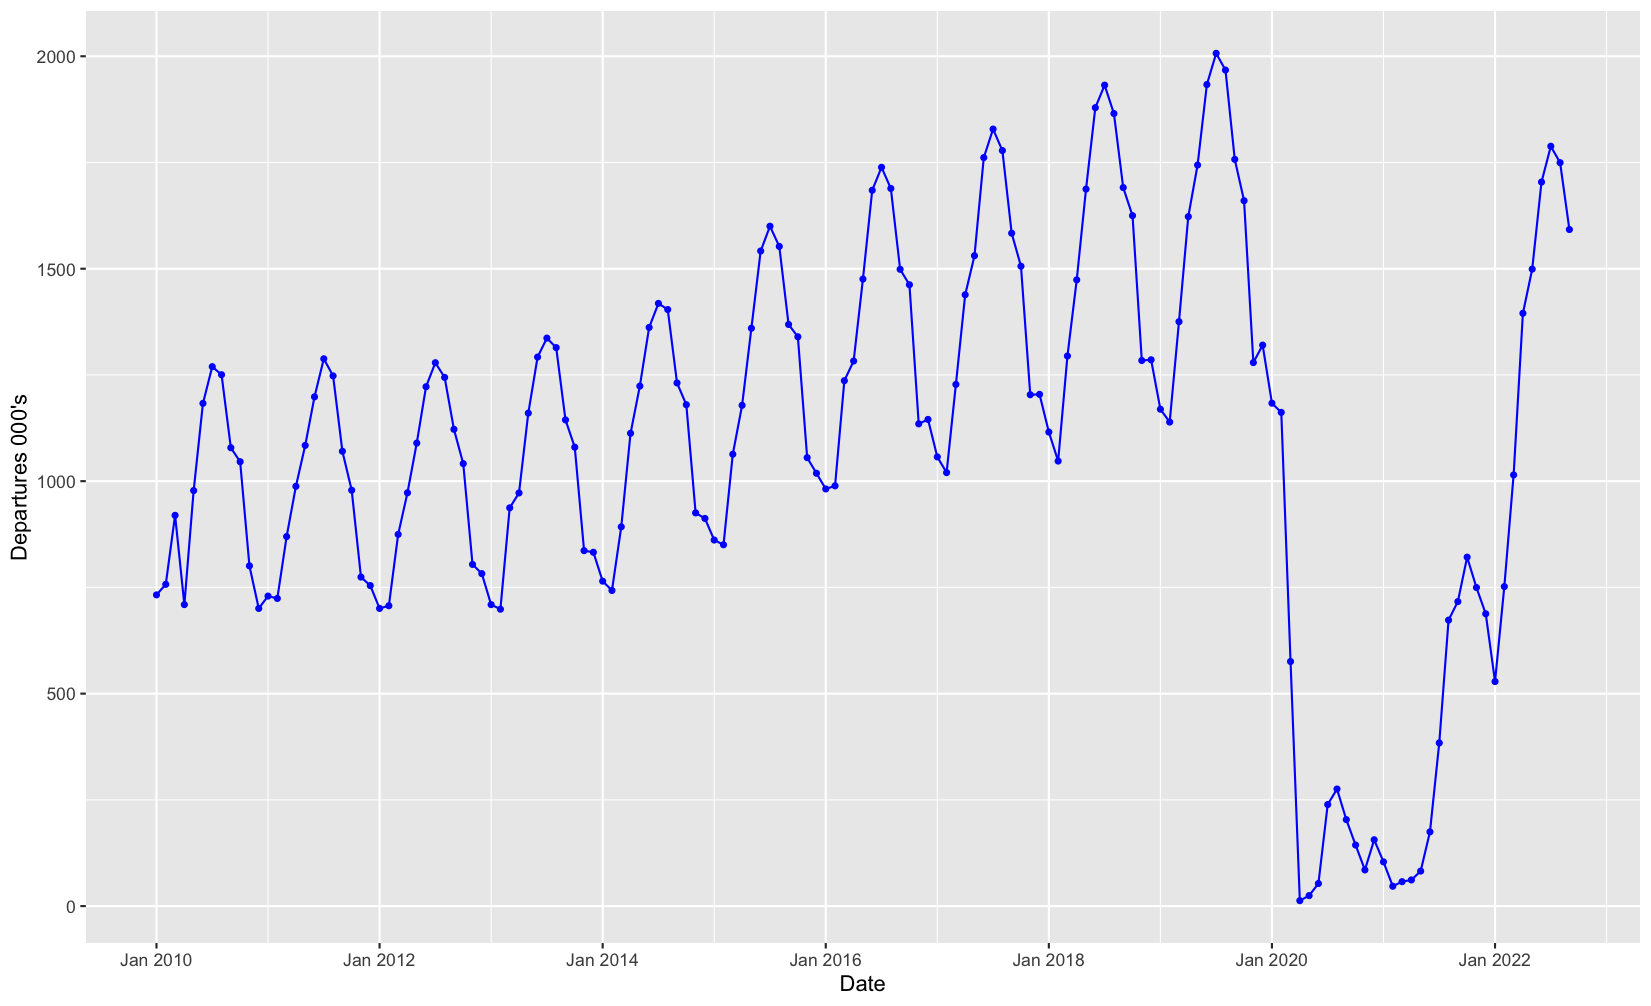
\includegraphics[width=1\textwidth]{ts_departs.png}
    \caption{Departures from Irish airports by month}
    \label{fig:ts_departs}
\end{figure*}

\subsection{Descriptive Statistics}

In this section, I estimate and analyse time series models based on monthly observations of departures from Irish airports.  The time series data itself is the only input into this analysis, no explanation in other variables is available from the data set given and the models I use do not look for one, instead looking to capture and then to understand the other

Data was downloaded in the file named \textit{Departure.csv}.  The file has 153 observations of the numbers in every calendar month of passengers departing from all Irish airports, reported in thousands.  

A simple graph of the departures against dates in figure~\ref{fig:ts_departs} gives a visual summary behaviour that we should aim to understand and forecast. In later sections, I use different time series tools to test, model and forecast these numbers and attempt to evaluate how they can be used in practise.  

I manually checked that there was one for every single month from and including January 2010 to and including September 2022, with all those months having one observation. No NA or otherwise unreadible results not suitable for numerical analysis were found in a visual inspection of this data. 

To allow processing with the specialist R libraries for time series, I transformed the data into a \textit{ts} object defined in the library \textit{tseries}.  Apart from the observations, the start and end dates were included in the definition, along with their frequency of 12 i.e. monthly.  

%\begin{figure}[htbp]
%\centerline{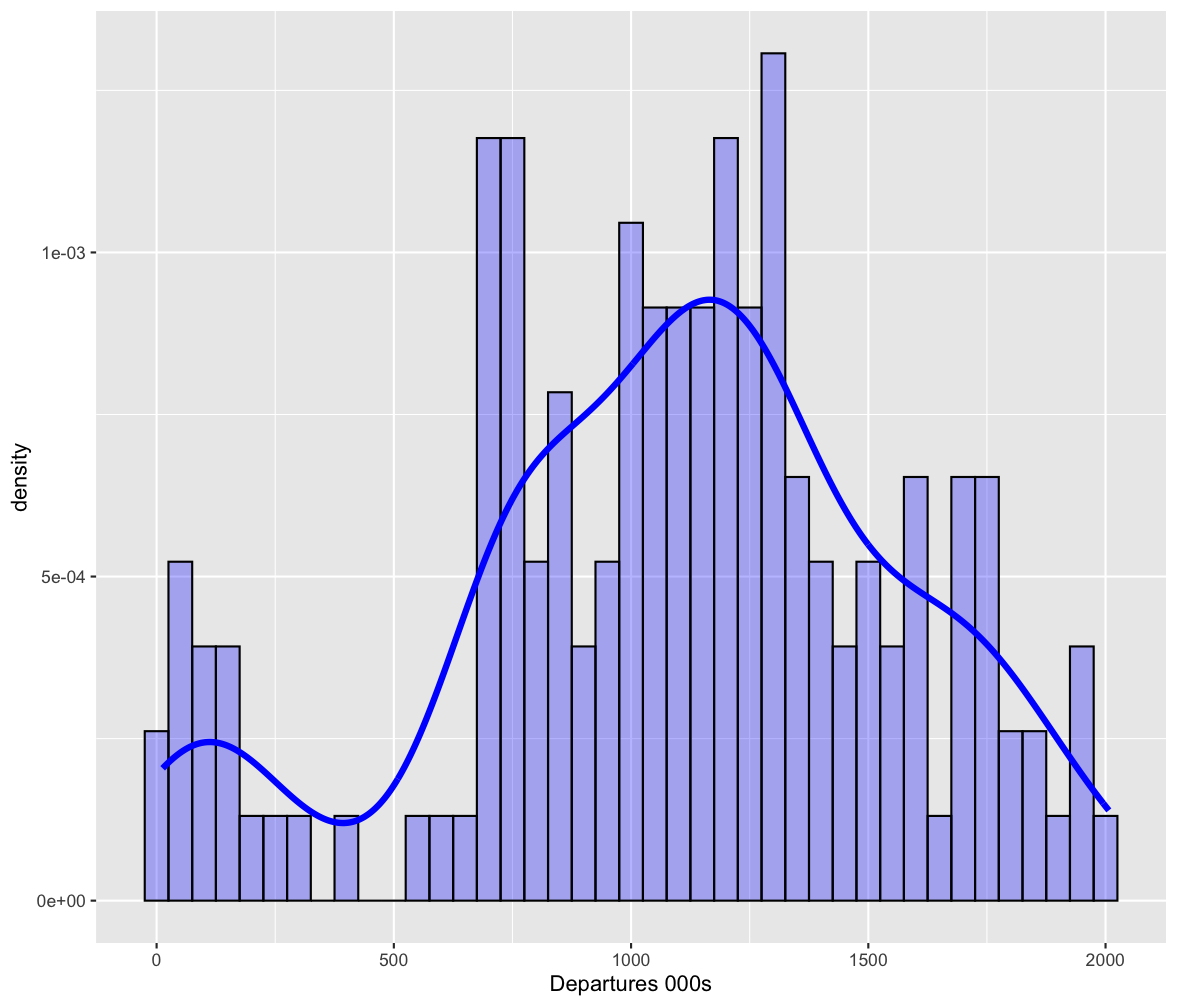
\includegraphics[scale=0.2]{density.png}}
%\caption{Histogram and density function of departures}
%\label{fig:density}
%\end{figure}

Behaviour in the data was visible that we can use to understand and then to forecast the time series.  Four aspects in particular, I believe, we have to make modelling choices about: 

\subsubsection{Seasonality}Seasonality is clearly visible and the same pattern consistently shows in all years, with the summer holiday months of June, July and August showing the highest passenger numbers in each year, with January and February consistently the lowest.  For making decisions involving airport operations such as staffing or retail businesses, this behaviour is likely to be always relevant.  

\subsubsection{Trend and Cyclical Factors} While appearing level from 2010 to 2013, from 2013 to 2020, our chart of departures to time shows a pronounced growth trend, with minimum and maximum numbers each year increasing every year, reaching the peak value in the dataset of over two million in July 2019.  The growth may be tied to economic growth and increased population in Ireland over the period.   2010 saw the bailout of Ireland's government and banking sector by the ECB, IMF and European Commission, with severe unemployment and loss of consumer confidence.  After 2013, factors such as rising incomes across Europe, increasing population in Ireland and improved business conditions may explain the consistent rise over several years up until 2019.  Operating on a longer-term than the seasonality within the year, this behaviour would be important for longer term decision making such as building terminals and buying planes.  

\subsubsection{Pandemic Shock}
The COVID19 pandemic's impact is clear in the first quarter of 2020, as the disease spread from China to Europe.  By April 2020, traffic at Heathrow airport in London was down by 97\% and some 2.7 billion workers, 81\% of the global workforce were under some form of lockdown \cite{tooze21}.  The economic fallout from the pandemic were all apparent when the departures numbers had a rapid fall in Q1 of 2020 to their low point in this dataset in April 2020 of only 12,800.  

Shocks like this to air travel are much rarer and hence much harder to plan for or model.   One such was the grounding of air travel and slow recovery after the 9/11 terrorist attacks in 2001.  Another was the outbreak of SARS, the first major coronavirus epidemic in 2004 and its spread through air travel\cite{greenfeld06}.  However, the deaths and disruption have probably been unique since the global influenza pandemic of 1918.  Pandemic insurance was offered by Munich Re but demand was very low and not part of regular operations planning. For our models then, this may not be something which can be incorporated.  

\subsubsection{Recovery}

Post-pandemic recovery seems to have seen different behaviour from the crisis conditions of the first few months of 2020, which saw the lowest value in the time series with 12,800 departures in April.  The remainder of 2020 showed departures remaining well below previous values, but peaking in the summer months as before, but reaching a maximum level for the year at only 275,500 in August.  

Unemployment had risen substantially everywhere in the early stages of the pandemic, but emergency welfare payments soon began to provide financial support.  From that low base, 2021 saw a partial recovery back to about half 2019 numbers by the autumn, peaking at 821,000 departures in October compared to 1,660,000 in October 2019.  Starting from a lower point than before, 2022 shows an annual maximum in the summer months of some 1,788,200, close to the highest observations recorded in 2016 and 2017.  This may be explainable by the economic rebound, as money saved during the pandemic is spent and as travel becomes possible again without onerous testing and quaratine.  

To me, this points towards the effect of the pandemic largely fading away and the regular seaonality and cyclical behaviour returning instead.  

\subsubsection{Descriptive Statistics}

Descriptive statistics were calculated.  The median and mean departures per month were 1,134,900 and 1,088,600 travellers per month.  Skewness was estimated for all observations at around -0.43, so leading to the right and kurtosis as 2.89, so with the central peak and tails close although not matching those of the normal distribution, as shown in the histogram in figure~\ref{fig:density}.  

The observations were grouped by calendar year and a box plot generated for each, as shown in figure~\ref{fig:boxplot}.  This highlights the upward trend 2013--2019 and the discontinuity and possible non-stationarity between 2019, before the pandemic, the impact of the pandemic in 2020, and then the strong recovery in departures in 2021 and 2022.    

A number of t-tests were performed on these sub-samples.  One rejected the two-sided null-hypothesis of equality between the mean of departures for calendar 2013 and 2019 with p.value of 7.696756e-05. A second, also rejected equality of means for 2019 and 2020, the year of the pandemic crisis.  A third rejected mean equality for the means for 2020 and 2022, the year that looks to be the second year of the recovery.  All results reinforce the idea that we face three distinct periods in our time-series sample data.  

\subsection{Exponential Smoothing}
\label{sec:exp}

Common solutions for forecasting are either exponential smoothing models that I cover in this section or ARIMA models that I discuss below in the next section~\ref{sec:arima}.  The treatment here closely follows \cite{fpp2} chapter 7.  

Given that our visualisation of the time series shows a what is likely to be a trend and seasonality, a sensible starting point is an exponential smoothing model that combines both these with a random element, namely the Holt-Winter (hereafter `HW') model in its additive form i.e. from \cite{fpp2}, section 7.3: 

\begin{equation}
\hat{y}_{t+h|t}=\ell_{t} + hb_{t} + s_{t+h-m(k+1)}
\end{equation}

\begin{equation}
\label{eq2}
\ell_{t} = \alpha(y_t - s_{t-m}) + (1-\alpha)(\ell_{t-1} + b_{t-1})
\end{equation}

\begin{equation}
\label{eq3}
b_t = \beta^{*} (\ell_t - \ell_{t-1}) + (1-\beta^{*})b_{t-1}
\end{equation}

\begin{equation}
\label{eq4}
s_t = \gamma(y_t - \ell_{t-1} - b_{t-1}) + (1-\gamma)s_{t-m}
\end{equation}

where $\alpha$ is the smoothing parameter for the level, $\beta$ for the trend and $\gamma$ for the seasonal adjustment component.  $\ell_t$, the smoothed series at $t$, $y_t$ the raw observed value of the series at $t$, h the number of periods ahead we are forecasting for, $b_t$ the estimated trend component at $t$, 

The level equation~\ref{eq2} shows a weighted average of a seasonally-adjusted observation in the first part and a non-seasonal component forecast as at $t$.  

The trend equation~\ref{eq3} shows how the current estimate of the trend $b_t$ is specified as a weighted average of the change in the smoothed series and the last value of the trend component.  

The seasonal equation~\ref{eq4} shows an average weighted by $\gamma$ between the current seasonal index component and the seasonal index of the same season $m$ time periods ago.

A damping parameter $\phi$ was included in the model by default, to prevent unlimited growth in the trend component. 

With ETS, solutions are estimated so as to minimise the sum of squared residuals of the model.  

Using the ETS function from the \textit{forecast} library, with the \textit{model = `ZZZ'} option allowing the software to automatically select the type, whether additive or multiplicative, for the error term, the trend and the seasonality components respectively, the system chose an additive model \textit{departs\_fit1} for all rather than multiplicative.  This was in line with prior expectations, as the graphical representation of the time series shows no noticeable increase in variance in the years before the arrival of the pandemic.  

The model \textit{departs\_fit1} scores an AIC corrected for small sample bias, AICc, of 2235.89 and Root Mean Squared Error (`RMSE') of 105.35.  The smoothing parameters were $\alpha = 0.9999$, $\beta = 0.1413$ and $\gamma = 1 \times 10^{-4}$.  A damping component was estimated with $\phi = 0.8$.  The same parameter estimates and scores came from running the ETS function with the same inputs but with the model explicitly set as additive for all components i.e. `AAA'.  

A third model without a damping parameter was also run, \textit{departs\_fit3}.  This generated worse scores than the earlier \textit{departs\_fit1} model, with AICc of 2245 compared to 2235 and RSME at 109.567 instead of 105.35.  

Forecasts were generated for 8 months past the end of the dataset.  The model \textit{departs\_fit1} with a damping parameter for the trend specified generated a range of forecasts of 746.3 to 2331.54 with a point forecast of 1538.9.  The model \textit{departs\_fit3} with the same setup except for no dampening, shows a higher point forecast 1904.69 and a wider range of 941.48 to 2867.9.  

Running \textit{checkresiduals} on \textit{departs\_fit1} shows a statistically significant autocorrelation of current against values with lag of 1.  The ACF, shown in figure \~ref{fig:ETSresiduals} also shows significant correlations around 23 and 24 months. A Box-Ljung test reinforces this by rejecting the null hypothesis of no autocorrelation with a p-value of 0.0001575.  A Jarque-Bera test rejects normality also, with a p-value near zero. 

\begin{figure}[htbp]
\centerline{\includegraphics[scale=0.25]{ETSresiduals.png}}
\caption{Testing residuals from our ETS model}
\label{fig:ETSresiduals}
\end{figure}

All this points to information not captured by the chosen model here still to be captured by some different models instead. 

\subsection{SARIMA Models}
\label{sec:arima}

In this section, I work to fit a model of the SARIMA (Seasonal Autoregressive Integrated Moving Average) type to the time series data.  While the exponential models fit trend and seasonality measurements, the ARIMA class focuses on identifying and estimating relationships between values of the time series at different times.  The treatment here largely follows \cite{fpp2} chapter 8.  

To begin, we can take first differences of our time series until it is stationary.  The function \textit{ndiffs} from R library \textit{forecast} tests for stationary in the time series, whether its properties depend on the time of observation:  In this case, the tests, using each of the three options available, namely a KPSS, Augmented Dickey-Fuller and  Phillips-Perron all return a zero value, indicating that the time series is stationary and does not need differencing before applying an ARIMA model.  

Doing the \textit{nsdiffs} test, applying the same logic but at time lags matching the seasonality of every 12th value in the case of our monthly data, returns a value of 1, showing non-stationary between every 12th observation in our series.  Together the two test results indicate that our data can be represented by a model of the form ARIMA(p,0,q)(P,1,Q)[12]. 

We may then continue on to plot the autocorrelation and partial autocorrelation functions of the time series, shown in figure~\ref{fig:Acf} and ~\ref{fig:Pacf}.  The ACF plot shows the correlation of the time series with its own past values: Here, several lag intervals show statistically significant levels different from zero of correlation with a gradual reduction over time, which points to a model with one or more autoregression terms, showing that previous observations in our time series have an influence on our current observation.  

\begin{figure}[htbp]
\centerline{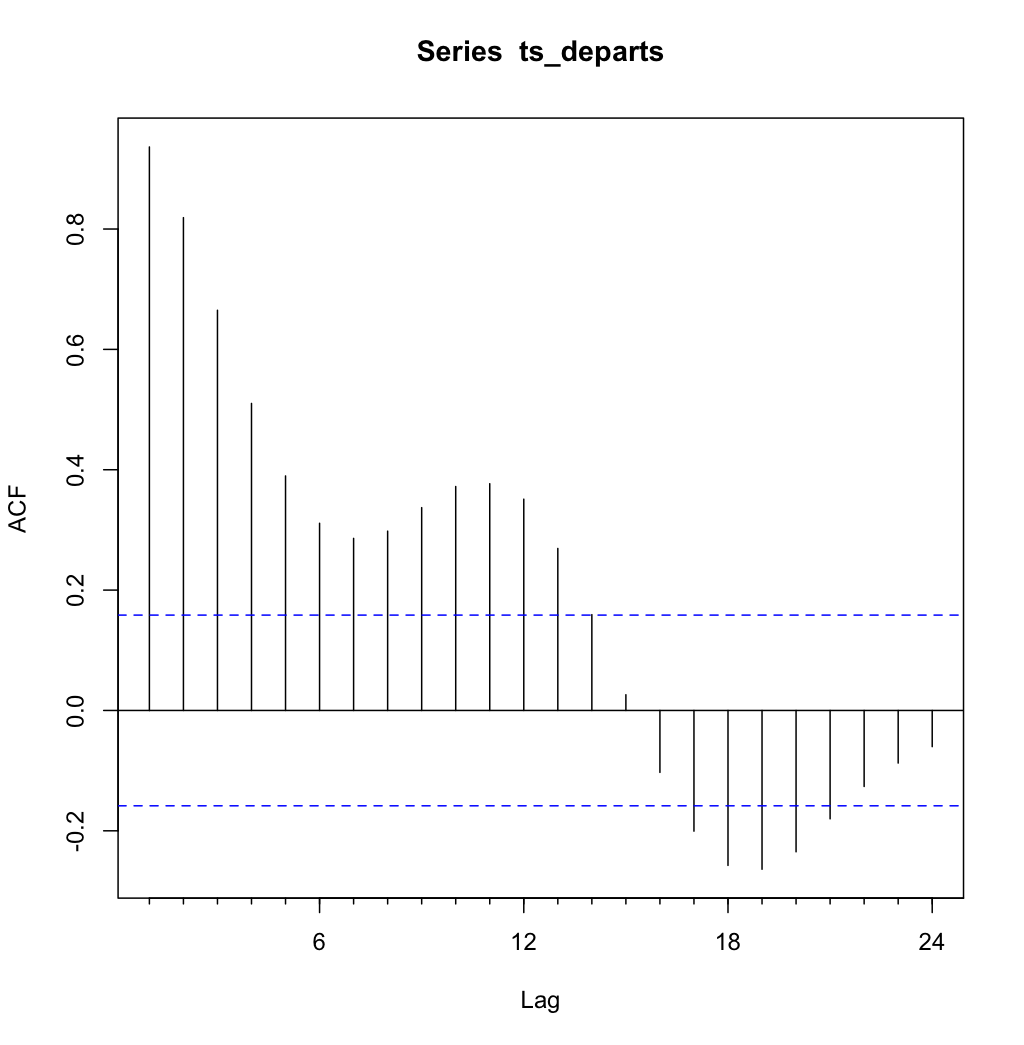
\includegraphics[scale=0.25]{Acf.png}}
\caption{ACF plot}
\label{fig:Acf}
\end{figure}

The PACF graph shows the correlation between the time series and values at each time lag not explained by any lower order autocorrelations.  The large and statistically significant partial autocorrelations at the lags of 1, 2, 3 and 5 are visible the PACF may indicate autoregression at those lags.  The significant autocorrelations at lags of 12 and above may indicate AR or MA processes among the same months' values from different years also.  

\begin{figure}[htbp]
\centerline{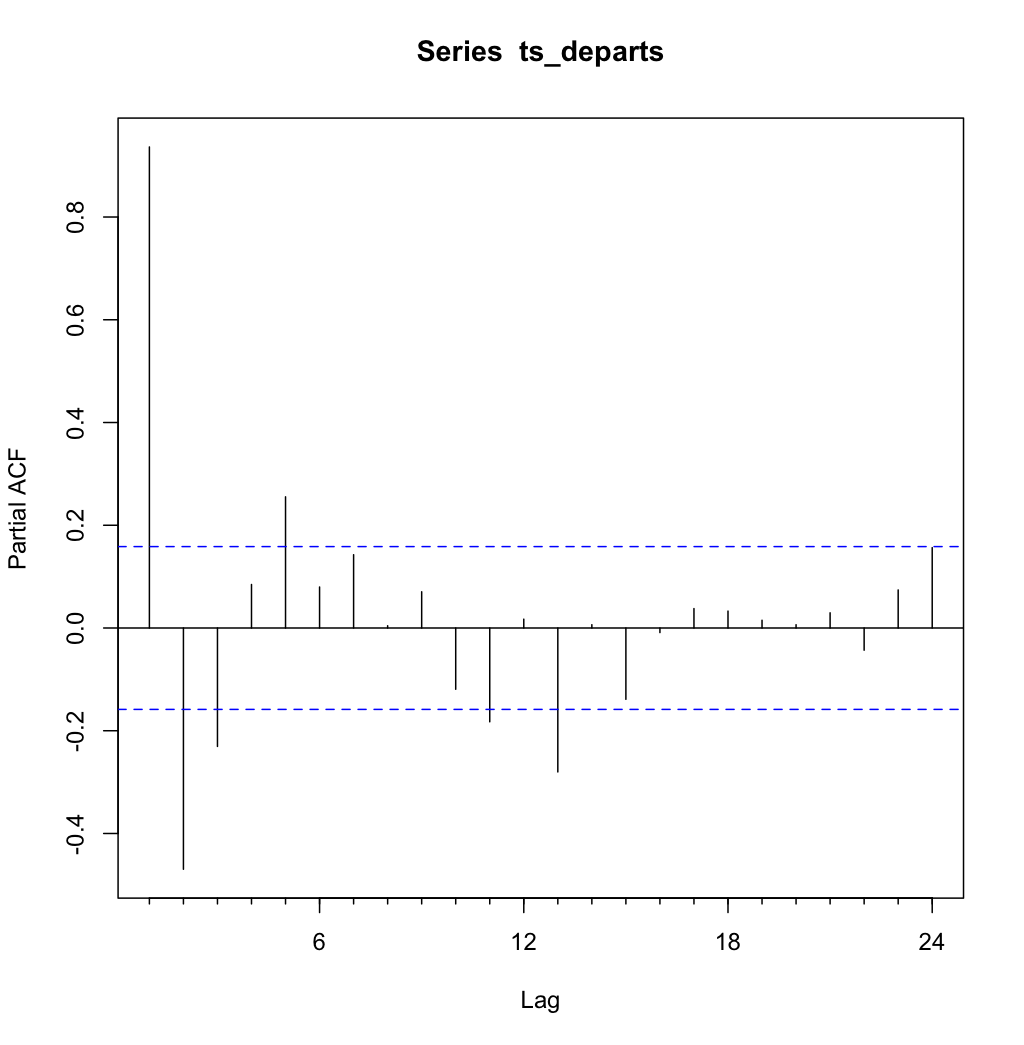
\includegraphics[scale=0.25]{Pacf.png}}
\caption{PACF plot}
\label{fig:Pacf}
\end{figure}

Proceeding to test and select from a number of possible SARIMA models, we may use the \textit{auto.arima} function, again from the \textit{forecast} library, for an automated search.  Given the large number of possible model specifications, searches for the best fit as determined by the AICc score, with the stepwise flag set to FALSE to specify the an exhaustive search and start.p and start.q both equal to 1 so as to search for the most models possible.  This returns a model specification of ARIMA(2,0,0)(0,1,1)[12]  

Looking at the residuals with the \textit{checkresiduals} function, we can test if the errors left after applying our SARIMA model to the time series show any systematic structure not captured by the model.  The plot is shown in figure~\ref{fig:SARIMA_residuals} and the lack of any statistically-significant autocorrelations would support our hope that the residuals behave like white noise. 

\begin{figure}[htbp]
\centerline{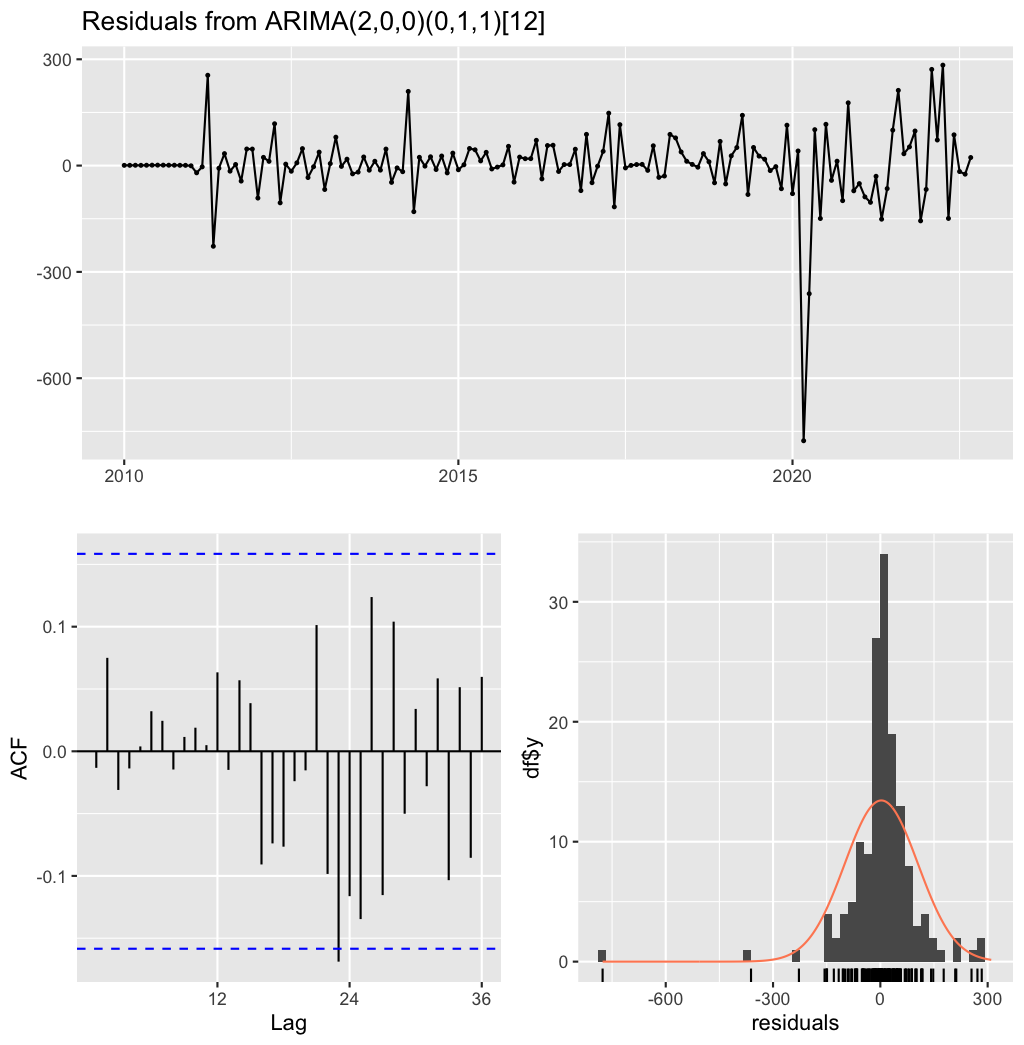
\includegraphics[scale=0.25]{SARIMA_residuals.png}}
\caption{Testing residuals from our SARIMA model}
\label{fig:SARIMA_residuals}
\end{figure}

Running a Ljung-Box test, the null hypothesis of independence among the residuals is also upheld, with the p-value of 65.94\%, again supporting the view that no autocorrelation and hence no systematic predictability remains within the residuals to capture in an updated version of our model.  

% Plotting the data
% Transform the data if necessary to stabilise the variance
% Check residuals by plotting their ACF and do a Box Ljung test
% Once residuals look like white noise, calculate the forcast values

\subsection{Simple Time Series Models}

decomposition models

\section{Applying a Forecasting Model}

%\begin{figure}[htbp]
%\centerline{\includegraphics[scale=0.5]{events_tests_1.png}}
%\caption{Price pre- and post-tweet}
%\label{event1}
%\end{figure}

\section{Logistic Regression for Analysing a Bank Marketing Campaign}

In this section, I analyse a dataset estimated over several years from the records of a Portuguese bank of the characteristics of a population of consumers and their interactions with the bank.  I relate this data to the customers decision to purchase or not a bank product by estimating and testing a logistic regression model   

\section{Understanding the Dataset}

The dataset consists of records derived from the dataset used by Moro et al.\cite{moro14}.  The file provided, \textit{Bank.csv} provides 45,211 records each with observations of 17 variables which we can use to analyse the purchase decision.  

Most of these variables are categorical variables, namely \textit{job, marital status, education, default , housing, loan, contact, previous outcome}.  Also included was \textit{y}, the outcome variable.  These have two or more discrete values, all known, with no numerical meaning or ranking among the different values: All these were converted using R to what it calls factor variables.  The numerical variables were not transformed.  All variables were imported into the dataframe \textit{bank}, which is not updated afterwards, and the cleaned and transformed values were added to the dataframe{bank\_clean}.  

Below, I have graphed the variables, trying to display visually and by calculating some descriptive statistics, if we can detect any signficant difference between the values of these variables between the cases with 'yes' and 'no' outcomes.  Violin plots are used to summarise the the numerical variables across the 'yes' and 'no' populations.  Code was adapted for these from \cite{chang19} \S 6.8,6.9. 

\subsection{Y} 

The variable $y$ is a variable indicating, yes or no, whether the client has subscribed for the bank product.  This is the dependent variable that we would expect to be able to try to explain using the other independent variables in the dataset.  This binary variable was converted into the R factor variable \textit{y\_factor} with values 'yes' and 'no'.  

One important fact to note immediately is that the observations are split into 39,922 'no' and 5,289 'yes' observations.  So, calculating 5289/(39922+5289)=  0.1169848, we see that approximately = 11.7\% of the observations are for 'yes' cases.  This is close to the 12.37\% rate of success in the original study\cite{moro14}.  As Moro et al. observe, this means that the dataset is unbalanced between the 'yes' and 'no' cases.  A naive estimator with no logic that just predicts 'no' in every case will still be correct about 88.3\% of the time.   This is not uncommon but requires adaptations in our model training and interpretation, described in detail in section~\ref{sec:imbalance} below.  

\subsection{Age}

In our violin plot in figure~\ref{fig:graph1age}, we see the distribution of the age variable in two separate buckets for 'yes' and 'no' customers.  The white dot shows the median.  The black area shows the box plot, with top and bottom edges at 75 and 25 percentile levels.  The results show some differences, with higher mean but lower median for 'yes' and significantly more skew and kurtosis for 'yes'.

\begin{figure}[htbp]
\centerline{\includegraphics[scale=0.25]{graph1age.png}}
\caption{Age in yes and no observations}
\label{fig:graph1age}
\end{figure}

\subsection{Balance}

As shown in our violin plot in figure~\ref{fig:graph3balance}, the 'yes' population has bigger relationshiop balance, with mean 1804 v 1303 EUR and median 733 v 417 EUR. 'yes' population also has far fewer zero or very low balance values than 'no'.  

\begin{figure}[htbp]
\centerline{\includegraphics[scale=0.25]{graph3balance.png}}
\caption{Balance in yes and no observations}
\label{fig:graph3balance}
\end{figure}

\section{Duration}

As shown in figure~\ref{fig:graph4duration} for the duration of the previous contact with the bank, 'yes' has fewer short conversations, a mean 537 seconds (about 9 mins) v 221 (under 4 mins) for 'no', median value of 426 v 164 i.e. 7 minutes compared with 2.5

\begin{figure}[htbp]
\centerline{\includegraphics[scale=0.25]{graph4duration.png}}
\caption{Duration in yes and no observations}
\label{fig:graph4duration}
\end{figure}

\section{Campaign}

The 'yes' population has lower number of contacts during this campaign, mean - 2.14 v 2.85.  The distribution is shown in figure ~\ref{fig:graph5campaign}.

\begin{figure}[htbp]
%\centerline{\includegraphics[scale=0.25]{graph5campaign.png}}
\centerline{\includegraphics[scale=0.25]{graph5and6.png}}
\caption{Campaign in yes and no observations}
\label{fig:graph5campaign}
\end{figure}

\subsection{Previous}

The 'yes' population saw more contacts before this campaign, 1.17 v 0.5, but the median for both subsets is zero contacts before this campaign.  The graph is shown in figure~\ref{fig:graph6previous}.  

%\begin{figure}[htbp]
%\centerline{\includegraphics[scale=0.25]{graph6previous.png}}
%\caption{Previous in yes and no observations}
%\label{fig:graph6previous}
%\end{figure}

\subsection{Month and Day}

Since the original dataset has observations from over five years of data, the date variables for the last contact offer the potential for finding seasonality in the data.  For the month, we might expect to see seasonal effects, with consumers spending most during summer holidays and the Christmas period, or spending on a new car typically in the first quarter, for education fees in August and September.  Any of these may lead to drawdowns of saving rather than new saving, so to 'no' in our caes here and lead instead to savings through the bank's offering at other times of the year.  The month was converted to a factor variable and retained for our model.  

For the day of the month, there are many values for a calendar day from 1 to 31, which could make for a lot of extra categorical variables.  Also, these numbers may be for different days of the week in different months and years.  Without more date data, the day was considered as likely to be irrelevant and not brought into the modelling analysis.   

The distributions of observations by month for both the 'yes' and the 'no' populations are shown in 
figure~\ref{fig:graph7month}.  In the 'yes' population, Feb, Mar, Apr, Oct appear as a bigger proportion than in 'no'.  May is also much bigger in the 'no' population.  

\begin{figure}[htbp]
\centerline{\includegraphics[scale=0.25]{graph7month.png}}
\caption{Months in yes and no observations}
\label{fig:graph7month}
\end{figure}

\subsection{Job}

Figure~\ref{fig:graph8job} shows the breakdown of job categories by 'yes' and 'no' population.  We can notice that the 'yes' population has a lower proportion of blue-collar, more retired and some more students.   

\begin{figure}[htbp]
\centerline{\includegraphics[scale=0.25]{graph8job.png}}
%\caption{Job category in yes and no observations}
\label{fig:graph8job}
\end{figure}

\subsection{Other Characteristics}

Marital status, education, figure~\ref{fig:graph9and10}


\begin{figure}[htbp]
\centerline{\includegraphics[scale=0.15]{graph9and10.png}}
%\caption{Job category in yes and no observations}
\label{fig:graph9and10}
\end{figure}


\begin{figure}[htbp]
\centerline{\includegraphics[scale=0.15]{graph11and12.png}}
%\caption{Job category in yes and no observations}
\label{fig:graph11and12}
\end{figure}

\begin{figure}[htbp]
\centerline{\includegraphics[scale=0.15]{graph13and14.png}}
%\caption{Job category in yes and no observations}
\label{fig:graph13and14}
\end{figure}

\section{Previous Outcome}

\begin{figure}[htbp]
\centerline{\includegraphics[scale=0.25]{graph15poutcome.png}}
%\caption{Job category in yes and no observations}
\label{fig:graph15poutcome}
\end{figure}

\subsection{Days since last contact}

The variable \textit{pdays} records the number of days since last contact with the customer.  Most observations almost 37,000 are equal to -1.  I assumed that these represent no recorded values, so replaced these with NA instead, making this the only variable in the dataset with any NA values.  The other 8,257 observations positive integers.

\subsection{Balance}
Note that balance, which might usually mean a relationship balance, the total balance summing across all accounts and loan balances across the relationship with the bank, is in the dataset but not in the document.  As it is potentially useful, I include it in the analysis here as a numerical variable.  


\subsection{Data Cleaning}

After the categorical variables were converted into R factor variables, these were dropped from the dataset.  Day was dropped also.  

\section{Building a Logistic Regression Model}

Binary outcome - to buy or not buy

\subsection{Stepwise Model Selection}

Move in both directions - full model ends up as the best based on the AIC data 

\section{Dealing with the Imbalanced Dataset}
\label{sec:imbalance}

\section{Applying the Model}

Odds ratios may be most useful in targeting the customers

\section{Example table} 

\begin{table}[htbp]
\caption{Reddit Posts: Polarity Percentiles }
\begin{center}
\begin{tabular}{|c|c|c|}
\hline
\textbf{Sentiment}&{\textbf{Textblob}}&{\textbf{VADER}} \\
%\cline{2-4} 
\hline
Positive& 39.9\%&42.4\%\\
\hline
Negative& 29.6\%&15.7\%\\
\hline
Neutral& 28\%&38.1\%\\
\hline
\end{tabular}
\label{tab2}
\end{center}
\end{table}

\section{Conclusions and Future Work}

Conclusions

Word Count = xxxx, excluding references

\bibliographystyle{IEEEtran}
\bibliography{dpnolan}

\end{document}